
\chapter{基于SSA的PCF函数式编译器概览} \label{sec:overview}

我们构建了一个从函数式语言PCF到LLVM IR的部分经过验证的编译器,并在Coq定理证明工具中
完成了编译算法和形式化验证的实现~\cite{chlipala2022certified}。
在本节中,我们主要是从高层次的角度介绍了这个编译器原型,省略了转换算法设计和证明定理的详细信息。
CPS转换及CPS到SSA转换的正确性通过源程序和目标程序之间的模拟进行形式化验证,
遵循第\ref{sec:compcertbackend}节中所介绍的CompCert后端的验证框架。
我们使用$\approx $表示语义保存性质。PCF、CPS和SSA的程序分别表示为$t_{pcf}$、$t_{cps}$和$t_{ssa}$。
通过对$t_{pcf}\approx t_{cps}$和$t_{cps}\approx t_{ssa}$的形式化证明,可以组合推导出$t_{pcf}\approx t_{ssa}$。
然后我们就得到了一个从PCF到SSA的经验证的编译过程。我们应用该经验证的编译过程,构建出一个编译器原型。
该编译器读取PCF程序,并经过图~\ref{overview}中所示的几个编译步骤生成LLVM IR程序。

\begin{figure}[htbp]
    \centering
    \vspace{2ex}
    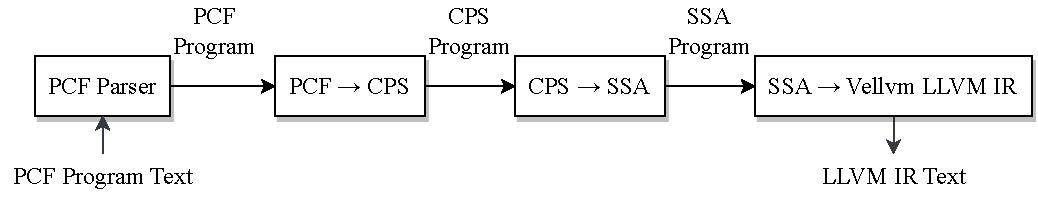
\includegraphics[width=0.8\linewidth]{figures/overview.pdf}
    \caption{PCF到LLVM编译链概览}\label{overview}
\end{figure}

\section{读入PCF文本}

使用PCF语法分析器(Parser)将文本形式的PCF程序提取为Coq中的结构化PCF代码项。
为了分析文本信息并提取PCF程序,获取源程序的语法结构至关重要。对于文本形式的PCF程序,
我们首先用词法分析器(Lexical Parser)将其解析为标记流(Tokens)。
随后,使用语法分析器(Syntax Parser)分析该标记流,生成Coq中的直接风格PCF程序项的抽象语法树。

\section{CPS转换}

如第\ref{sec:background}节中所言,函数式编程语言的编译器通常会将直接风格的程序转换为CPS形式,以获得显式的控制流。
我们已经得到了PCF程序的抽象语法树,但它是直接风格的程序,所以接下来需要使用CPS转换将其编译为CPS风格的程序。
将直接风格的PCF程序转换为CPS形式的算法主要由当前代码项和当前项被规约为某个值后要处理的下一个项决定。
另外,我们为直接风格及CPS风格的PCF语言定义了小步操作语义,并证明了CPS转换的前向模拟性质。
关于该CPS转换算法及其正确性验证的详细信息将在第\ref{sec:cpstrans}节和第\ref{sec:cpsforward}节中进行讨论。

\section{从CPS到SSA}

该编译链中最关键的部分是从CPS风格的函数式程序到目标SSA程序的转换及验证。
目标SSA语言是LLVM IR的简化版本,保留了其最基本的结构和程序语句。
通过该编译过程,输入的CPS程序项将被转换为一个包含主函数的SSA程序。
同样的,我们为这种SSA语言定义了小步操作语义,并证明了从CPS到SSA转换的前向模拟。
完成这一步证明后,我们将正向模拟组合起来,并完成了从源程序到SSA程序后向模拟的证明。
在第\ref{sec:cpsssatrans}节中将详细介绍该转换算法的设计和细节。
第\ref{sec:cpsssaforward}节中将进行CPS到SSA转换算法的形式化验证,并通过运行一个示例程序展示前向模拟的每一个关键步骤。

\section{从SSA到LLVM IR}

上一步中得到的SSA程序被转换为Vellvm中的抽象语法树,然后转换为LLVM IR程序文本。
在该编译链中,我们使用了经过验证的LLVM基础设施Vellvm~\cite{zakowski2021modular}。
利用其在Coq实现的LLVM IR的抽象语法树,我们可以进一步输出最终的LLVM IR程序。
由于我们使用的SSA语言是LLVM IR的简化版本,它保留了LLVM IR程序的基本结构,
可以方便地编译到Vellvm中的抽象语法树。这种SSA语言省略了LLVM IR中的大部分参数。
例如,函数定义在LLVM中非常复杂,有很多可选的参数,而本文中的SSA语言只保留了函数定义中必须指定的内容。
LLVM中的表达式类型多种多样,其中整数包括多种宽度的i16、i32等,
而本文的SSA语言简化为没有明确指定类型的无限宽自然数。
该编译过程的主要工作其实就是为这些被省略的参数选取正确的默认值。

\section{核心编译步骤的正确性验证}

我们为CPS转换和CPS到SSA的转换证明了正向模拟性质。将它们组合起来可以得到
从PCF源程序到SSA程序的正向模拟。我们还证明了SSA程序的确定性,
并利用该性质和正向模拟性质证明了PCF到SSA的反向模拟,即证明了$t_{pcf}\approx t_{ssa}$。

